%%% File-Information {{{
%%% Filename: template_bericht.tex
%%% Purpose: lab report, technical report, project report
%%% Time-stamp: <2004-06-30 18:19:32 mp>
%%% Authors: The LaTeX@TUG-Team [http://latex.tugraz.at/]:
%%%          Karl Voit (vk), Michael Prokop (mp), Stefan Sollerer (ss)
%%% History:
%%%   20050914 (ss) correction of "backref=true" to "backref" due to hyperref documentation
%%%   20040630 (mp) added comments to foldmethod at end of file
%%%   20040625 (vk,ss) initial version
%%%
%%% Notes:
%%%
%%%
%%%
%%% }}}
%%%%%%%%%%%%%%%%%%%%%%%%%%%%%%%%%%%%%%%%%%%%%%%%%%%%%%%%%%%%%%%%%%%%%%%%%%%%%%%%
%%% main document {{{

\documentclass[
a4paper,     %% defines the paper size: a4paper (default), a5paper, letterpaper, ...
% landscape,   %% sets the orientation to landscape
% twoside,     %% changes to a two-page-layout (alternatively: oneside)
% twocolumn,   %% changes to a two-column-layout
% headsepline, %% add a horizontal line below the column title
% footsepline, %% add a horizontal line above the page footer
% titlepage,   %% only the titlepage (using titlepage-environment) appears on the first page (alternatively: notitlepage)
% parskip,     %% insert an empty line between two paragraphs (alternatively: halfparskip, ...)
% leqno,       %% equation numbers left (instead of right)
% fleqn,       %% equation left-justified (instead of centered)
% tablecaptionabove, %% captions of tables are above the tables (alternatively: tablecaptionbelow)
% draft,       %% produce only a draft version (mark lines that need manual edition and don't show graphics)
% 10pt         %% set default font size to 10 point
% 11pt         %% set default font size to 11 point
12pt         %% set default font size to 12 point
]{scrartcl}  %% article, see KOMA documentation (scrguide.dvi)



%%%%%%%%%%%%%%%%%%%%%%%%%%%%%%%%%%%%%%%%%%%%%%%%%%%%%%%%%%%%%%%%%%%%%%%%%%%%%%%%
%%%
%%% packages
%%%

%%%
%%% encoding and language set
%%%

%%% ngerman: language set to new-german
\usepackage{ngerman}

%%% babel: language set (can cause some conflicts with package ngerman)
%%%        use it only for multi-language documents or non-german ones
\usepackage[ngerman]{babel}

%%% inputenc: coding of german special characters
\usepackage[latin1]{inputenc}

%%% fontenc, ae, aecompl: coding of characters in PDF documents
%\usepackage[T1]{fontenc}
\usepackage{ae,aecompl}

%%%
%%% technical packages
%%%

%%% amsmath, amssymb, amstext: support for mathematics
\usepackage{amsmath,amssymb,amstext}

%%% psfrag: replace PostScript fonts
\usepackage{psfrag}

%%% listings: include programming code
\usepackage{algpseudocode} 
\usepackage{algorithmicx} 
\usepackage{algorithm}
\usepackage{listings}

%%% units: technical units
%\usepackage{units}

%%%
%%% layout
%%%

%%% scrpage2: KOMA heading and footer
%%% Note: if you don't use this package, please remove 
%%%       \pagestyle{scrheadings} and corresponding settings
%%%       below too.
\usepackage[automark]{scrpage2}


%%%
%%% PDF
%%%

\usepackage{ifpdf}

%%% Should be LAST usepackage-call!
%%% For docu on that, see reference on package ``hyperref''
\ifpdf%   (definitions for using pdflatex instead of latex)

  %%% graphicx: support for graphics
  \usepackage[pdftex]{graphicx}

  \pdfcompresslevel=9

  %%% hyperref (hyperlinks in PDF): for more options or more detailed
  %%%          explanations, see the documentation of the hyperref-package
  \usepackage[%
    %%% general options
    pdftex=true,      %% sets up hyperref for use with the pdftex program
    %plainpages=false, %% set it to false, if pdflatex complains: ``destination with same identifier already exists''
    %
    %%% extension options
    backref,      %% adds a backlink text to the end of each item in the bibliography
    pagebackref=false, %% if true, creates backward references as a list of page numbers in the bibliography
    colorlinks=true,   %% turn on colored links (true is better for on-screen reading, false is better for printout versions)
    %
    %%% PDF-specific display options
    bookmarks=true,          %% if true, generate PDF bookmarks (requires two passes of pdflatex)
    bookmarksopen=false,     %% if true, show all PDF bookmarks expanded
    bookmarksnumbered=false, %% if true, add the section numbers to the bookmarks
    %pdfstartpage={1},        %% determines, on which page the PDF file is opened
    pdfpagemode=None         %% None, UseOutlines (=show bookmarks), UseThumbs (show thumbnails), FullScreen
  ]{hyperref}


  %%% provide all graphics (also) in this format, so you don't have
  %%% to add the file extensions to the \includegraphics-command
  %%% and/or you don't have to distinguish between generating
  %%% dvi/ps (through latex) and pdf (through pdflatex)
  \DeclareGraphicsExtensions{.pdf}

\else %else   (definitions for using latex instead of pdflatex)

  \usepackage[dvips]{graphicx}

  \DeclareGraphicsExtensions{.eps}

  \usepackage[%
    dvips,           %% sets up hyperref for use with the dvips driver
    colorlinks=false %% better for printout version; almost every hyperref-extension is eliminated by using dvips
  ]{hyperref}

\fi


%%% sets the PDF-Information options
%%% (see fields in Acrobat Reader: ``File -> Document properties -> Summary'')
%%% Note: this method is better than as options of the hyperref-package (options are expanded correctly)
\hypersetup{
  pdftitle={}, %%
  pdfauthor={}, %%
  pdfsubject={}, %%
  pdfcreator={Accomplished with LaTeX2e and pdfLaTeX with hyperref-package.}, %% 
  pdfproducer={}, %%
  pdfkeywords={} %%
}


%%%%%%%%%%%%%%%%%%%%%%%%%%%%%%%%%%%%%%%%%%%%%%%%%%%%%%%%%%%%%%%%%%%%%%%%%%%%%%%%
%%%
%%% user defined commands
%%%

%%% \mygraphics{}{}{}
%% usage:   \mygraphics{width}{filename_without_extension}{caption}
%% example: \mygraphics{0.7\textwidth}{rolling_grandma}{This is my grandmother on inlinescates}
%% requires: package graphicx
%% provides: including centered pictures/graphics with a boldfaced caption below
%% 
\newcommand{\mygraphics}[3]{
  \begin{center}
    \includegraphics[width=#1, keepaspectratio=true]{#2} \\
    \textbf{#3}
  \end{center}
}

%%%%%%%%%%%%%%%%%%%%%%%%%%%%%%%%%%%%%%%%%%%%%%%%%%%%%%%%%%%%%%%%%%%%%%%%%%%%%%%%
%%%
%%% define the titlepage
%%%

\subject{statistische Verfahren WS 2017/2018}   %% subject which appears above titlehead

%%% title
\title{Projekt 7 - Kriminalit\"at}

%%% author(s)
\author{Reda Ihtassine (155 685) \and
Ingo Sch\"afer (165 220)}

%%% date
\date{Jena, am \today{}}

% \publishers{}

% \thanks{} %% use it instead of footnotes (only on titlepage)

% \dedication{} %% generates a dedication-page after titlepage


%%% uncomment following lines, if you want to:
%%% reuse the maketitle-entries for hyperref-setup
%\newcommand\org@maketitle{}
%\let\org@maketitle\maketitle
%\def\maketitle{%
%  \hypersetup{
%    pdftitle={\@title},
%    pdfauthor={\@author}
%    pdfsubject={\@subject}
%  }%
%  \org@maketitle
%}


%%%%%%%%%%%%%%%%%%%%%%%%%%%%%%%%%%%%%%%%%%%%%%%%%%%%%%%%%%%%%%%%%%%%%%%%%%%%%%%%
%%%
%%% set heading and footer
%%%

%%% scrheadings default: 
%%%      footer - middle: page number
\pagestyle{scrheadings}

%%% user specific
%%% usage:
%%% \position[heading/footer for the titlepage]{heading/footer for the rest of the document}

%%% heading - left
% \ihead[]{}

%%% heading - center
% \chead[]{}

%%% heading - right
% \ohead[]{}

%%% footer - left
% \ifoot[]{}

%%% footer - center
% \cfoot[]{}

%%% footer - right
% \ofoot[]{}



%%%%%%%%%%%%%%%%%%%%%%%%%%%%%%%%%%%%%%%%%%%%%%%%%%%%%%%%%%%%%%%%%%%%%%%%%%%%%%%%
%%%
%%% begin document
%%%

\begin{document}

\pagenumbering{roman} %% small roman page numbers

%%% include the title
% \thispagestyle{empty}  %% no header/footer (only) on this page
 \maketitle

%%% start a new page and display the table of contents
\newpage
\tableofcontents

%%% start a new page and display the list of figures
\newpage
\listoffigures

%%% start a new page and display the list of tables
\newpage
\listoftables

%%% display the main document on a new page 
\newpage

\pagenumbering{arabic} %% normal page numbers (include it, if roman was used above)

%%%%%%%%%%%%%%%%%%%%%%%%%%%%%%%%%%%%%%%%%%%%%%%%%%%%%%%%%%%%%%%%%%%%%%%%%%%%%%%%
%%%
%%% begin main document
%%% structure: \section \subsection \subsubsection \paragraph \subparagraph
%%%

\label{sec:ein}
\section{Einleitung}
\input{chapters/introduction}
\newpage

\label{sec:mat}
\section{Material und Methoden}
\subsection{Material}
Cornwell und Trumbull (1994)\footref{ftn:cut}, sch\"atzten ein Wirtschaftsmodell der Kriminalit\"at unter Verwendung von Daten aus 90 Counties in North Carolina zwischen 1981 und 1987. 
Becker (1963) und Ehrlich (1973)\footnote{Ehrlich I. 1973. Participation in illegitimate activities: a theoretical and empirical investigation. Journal of Political Economy 81: 521–567.\label{ftn:ehr}} unter anderem folgen dem empirische Modell, welches die Kriminalit\"atsrate misst und sich dabei auf eine Reihe von Variablen bezieht. 
Dazu geh\"oren auch solche Variablen, wie z.B. die Angst eine Straftat zu begehen oder auch Variablen, die messen wie oft der T\"ater danach wieder straffrei geblieben ist.
Diese Kriminalit\"atsrate ist ein FBI-Index, der das Verh\"altnis zwischen Anzahl der Verbrechen und der Kreisbev\"olkerung berechnet\footnote{Vgl.: Badi H. Baltagli, estimating an economic model of crime using panel data from North Carolina, journal of applied econometrics, S.: 543 f.}. \\
In dieser Arbeit jedoch werden nicht alle diese Daten zur Ermittlung eines geeigneten Modells genutzt.
Hier folgt eine Beschreibung des Datensatzes: \\

Der Datensatz ist in einer .csv-Datei gespeichert.
In ihr sind die unterschiedlichen 90 Counties von North Carolina zeilenweise aufgelistet.
Die Spalten sind (m\"ogliche) Eigenschaftsvektoren.
Alle Eigenschaftsvektoren sind logarithmisch mit Ausnahme der Region, die eine Dummy-Variable ist. \\
Die erste Spalte beinhaltet die Zielgr\"o\ss{}e \textit{crimes}, also die Anzahl aller Straftaten in dem jeweiligen County \"uber den Zeitraum von 1981-1987. 
\par\smallskip
Weiterhin wurde die Arrestwahrscheinlichkeit $P_A$ hinzugef\"ugt. Sie berechnet sich aus 
\begin{equation}
P_A = \frac{\text{Arrestierungen}}{\text{Delikte}}
\end{equation}
Sie wird abgek\"urzt \textit{prbarr} geschrieben. \newline
\par\smallskip
Daneben gibt es auch die \"Uberzeugungswahrscheinlichkeit $P_C$. Sie gibt das Verh\"altnis zwischen tats\"achlichen Arrestierungen und den gestandenen Straftaten an und wird daher berechnet mit 
\begin{equation}
P_C = \frac{\text{Anzahl tats\"achlicher Arrestierungen}}{\text{Anzahl gestandener Straftaten}}
\end{equation}
Sie wird bezeichnet als \textit{prbpris}. \newline
\par\smallskip
Eine weitere Eigenschaft ist die F\"ahigkeit des Countys ein Verbrechen auch zu ermitteln. In dem Datensatz spiegelt sich dies in der Variable \textit{polpc} wieder. Sie gibt das Verh\"altnis zwischen Anzahl der Polizisten zu der Bev\"olkerungsanzahl an. \newline
\par\smallskip
Ein weiteres wichtiges Merkmal ist die Bev\"olkerungsdichte (\textit{density}). Sie stellt das Verh\"altnis zwischen der Bev\"olkerungsanzahl und der Fl\"ache des Countys (in square miles) dar. \newline
\par\smallskip
Dar\"uberhinaus wird das Verh\"altnis von Minderheiten zu der Gesamtanzahl Einwohner in der Variable \textit{pctmin} ausgedr\"uckt. \\
\textit{pctymale} ist eine Eigenschaft, die den Anteil der jungen m\"annlichen Bev\"olkerung zur Gesamtbev\"olkerung anzeigt. \\
\par\smallskip
Die letzten f\"unf Variablen geben den durschnittlichen Bruttolohn in den Bereichen Baugewerbe (\textit{wcon}), Staatsangestelle (\textit{wsta}), Dienstleistungssektor (\textit{wser}), Handel (\textit{wtrd}) und Bankgesch\"aften (\textit{wfir}) wieder.
\par\medskip

\subsection{Methoden}
\label{sec:met}
Um ein geeignetes Modell aus den oben beschriebenen Merkmalen zu finden, wurden f\"unf unterschiedliche Herangehensweisen vorgeschlagen, um ein Modell zu finden, das m\"oglichst geringe Fehler aufweist.
\begin{itemize}
	\item explorative Herangehensweise (ausprobieren)
	\item Vergleich aller Modelle mit nur einem Merkmal
	\item Verwendung von step() und anschlie\ss{}ende Minimierung des Modells
	\item strukturierte Suche nach einem geeigneten Modell
	\item Verwendung von cor()
\end{itemize}
Am Ende einer jeden Herangehensweise wurde ein bestes Modell vorgschlagen. Diese wurden dann anschlie\ss{}end miteinander verglichen, um ein bestm\"ogliches Modell zu bestimmen.
\par\smallskip

\noindent
Haupts\"achlich wurden zwei G\"utekriterien verwendet, um verschiedene Modelle miteinander vergleichen zu k\"onnen.
\par\smallskip
Zum einen \textit{Akaikes Information Criterion} (AIC), welches die logarithmische Fehlerabweichung des Sch\"atzers $ln(\underline{\hat{\Theta}}_n)$ mit der Anzahl der verwendeten Merkmale $p$ bestraft. \\
\begin{equation}
\text{AIC} := -2*ln(\underline{\hat{\Theta}}_n) + 2p
\label{eq:aic}
\end{equation}  
Je kleiner also der erhaltene Wert ist, desto besser sei das untersuchte Modell. \\
Der Faktor $2$, der hier in Formel (3) auftritt, kann mit einem beliebigen Wert $n, n\in \mathds{N}$ belegt werden. In dieser Arbeit wurde er allerdings dauerhaft auf $2$ belassen. \\ 
AIC spiegelt den Kompromiss zwischen Verbesserung der Modellanpassung durch erh\"ohte $p$ und erh\"ohte Ungenauigkeit durch Sch\"atzung vieler Parameter wider.
\par\smallskip
In einigen F\"allen wurde auch die \textit{Devienz} betrachtet, um die G\"ute mehrerer Modelle miteinander zu vergleichen. \\
Hier geht man von einem saturierten Modell aus. Dies ist das komplexeste Modell f\"ur einen Datensatz, dass durch Erh\"ohung der Parameterzahl erzeugt werden kann. In vielen F\"allen hat das saturierte Modell daher so viele Parameter wie Beobachtungen. Falls Einflusvektoren mehrfach vorkommen, besitzt das saturierte Modell weniger Parameter. Das ist typischerweise der Fall f\"ur Experimente mit qualitativen Einflussgr\"o\ss{}en. \\
Hier wird die Likelihood-Quotienten-Statistik zum Vergleich eines Modells $M$ mit dem saturierten Modell 
\begin{equation}
T(\underline{Y}) = 2(l_{\text{saturiert}} - l_M)
\end{equation}
betrachtet. \\
Die Likelihood-Quotienten-Statistik ist asymptotisch  $\mathcal{X}^2$ - verteilt. Dabei ist $r$ die Differenz der Parameterzahlen. Deswegen funktioniert hier der Likelihood-Quotienten-Test nicht, da f\"ur $n \rightarrow \infty$ die Anzahl der Freiheitsgrade auch typischerweise unbeschr\"ankt w\"achst. \\
Die Gr\"o\ss{}e 
\begin{equation}
D(M) = 2(l_{\text{saturiert}} - l_M)
\end{equation}
hei\ss{}t Devienz des Modells $M$. \\
Dabei ist zu beachten, dass ein Modell $M$ ein geeignetes Modell ist, falls die Devienz von $M$ ungef\"ahr so gro\ss{} ist wie die ungef\"ahre Anzahl Parameter von $M$. \\
\begin{equation}
D(M) \approx n - |M|
\end{equation}
\par\medskip

Als anderes G\"utekriterium wurde das Quadrat der erwarteten Fehlerabweichungen (\textit{SPSE}) im Kreuzvalidierungsverfahren berechnet. \\
Dazu wurde der gesamte ausgew\"ahlte Datensatz in einen Trainings- und einen Testdatensatz aufgeteilt. Das "beste Modell" ist dasjenige, dass im Mittel den kleinsten gesch\"atzten erwarteten Prognosefehler liefert.
Dabei wird typischerweise eine l-fache Kreuzvalidierung durchgef\"uhrt: \\
Es gibt einen Testdatensatz $I = {1...n}$. Dieser wird in l etwa gleichgro\ss{}e Indexmengen $I_1, ..., I_l$ zerlegt. \\
In jedem j-ten Schritt wird ein $I_j$ als Testdatensatz gew\"ahlt. Alle anderen Indexmengen bilden den Trainingsdatensatz. \\
Nun wird der erwartete Prognosefehler gesch\"atzt: \\
\begin{equation}
\sum_{i \in I_j} (y_i - \underline{x}_i^{(M)^T} \underline{\hat{\beta}}^{(m-j)}})^2 = \hat{SPSE}_j^{(M)}
\end{equation}
Dabei ist $\underline{\hat{\beta}}^{(m-j)}$ die auf $I/I_j$ basierende Sch\"atzung. \\
Zuletzt werden alle Teilsch\"atzungen zu einer Sch\"atzung f\"ur SPSE zusammen kombiniert: \\
\begin{equation}
\hat{SPSE}^{(M)} := \sum_{j=1}^l (\hat{SPSE}_j^{(M)})
\end{equation}
Zu bemerken ist, dass jede Beobachtung einmal in einem Testdatensatz verwendet wird. Au\ss{}erdem ist die Abh\"angigkeit von der konkreten Zerlegung nur reduziert, aber nicht verschwunden. Es gibt einen Spezialfall, wenn $l=n$. Das hei\ss{}t, dass der gestamte Testdatensatz in $n$ Teildatens\"atze zerlegt wird. Jede Beobachtung wird mit der Prognose basierend auf $(n-1$ Beobachtungen verglichen. Dies ist auch bekannt als \textit{leave-one-out-cross-validation}. Als Faustregel empfiehlt es sich $l \approx 10$ zu w\"ahlen. \\
\par\bigskip

In der Simulationsaufgabe des Projektes sollte der Einfluss des Stichprobenumfangs auf die Genauigkeit der Approximation der tats\"achlichen Kovarianzmatrix des Maximum-Likelihood-Sch\"atzers durch die asymptotische Kovarianzmatrix untersucht werden\footnote{Dieser zweite Teil ist aus der Vorlesung}.
Dazu wurde zun\"achst ein m\"oglichst einfaches wahres Modell angenommen. Anhand dessen wurde aus dem gesamten Datensatz eine beliebig gro\ss{}e Teilmenge $T$ entnommen. Aus den Daten von $T$ wurde dann eine Designmatrix gebildet, die Grundlage f\"ur die darauf folgendenden Generierungen f\"ur Pseudozufallszahlen war. Standarm\"a\ss{}ig wurde die Gr\"o\ss{}e dieser zu untersuchenden Teilmenge auf $30$ gesetzt. (Der gesamte Datensatz umfasst 90 Subjekte.) Jedoch wurden auch viele andere Gr\"o\ss{}en \"uberpr\"uft. Aus der auf diese Art und Weise gebildeten Designmatrix, wurden nun wiederum unterschiedlich gro\ss{}e Stichproben ausgew\"ahlt und die daraus berechneten $\beta_0$ und $\beta_1$ Werte in einer weiteren Matrix gespeichert. Aus dieser Matrix wurden dann die Varianz und die Kovarianz f\"ur die tats\"achliche Kovarianzmatrix berechnet. \\
\par\smallskip
Da
\begin{equation}
F^{\frac{T}{2}}(\underline{\hat{\beta}}) (\underline{\hat{\beta}}_n - \underline{\beta})
\xrightarrow[n \rightarrow \infty]{d}
N(0,I)
\end{equation}
gilt, gilt f\"ur die Approximation von $\underline{\hat{\beta}}_n$ bei festem $n$:
\begin{equation}
\underline{\hat{\beta}}_n \approx N(\underline{\beta}, I^{-1}(\beta))}
\end{equation}
Die Kovarianzmatrix $\mathbb{X}$ ist die inverse Fisher-Matrix $I$. Daher hat $I(\underline{\beta})$ die kanonische Linkfunktion einfachen Gestalts
\begin{equation}
I(\underline{\beta}) = \mathbb{X}^T V \mathbb{X}
\end{equation}
Dabei ist $V$ eine Diagonalmatrix, welche in der Spur die Varianzen h\"alt.
Anhand dessen wurde die asymptotische Kovarianzmatrix berechnet.
Die daraus herausgehenden Resultate wurden dann bei einem kleiner werdenden $n$ auch immer geringer, sodass die Ergebnisse immer in Relation zueinander verglichen wurden. \\
Daher hat es sich angeboten eine Hilfsfunktionen \texttt{simulation()} zu schreiben, welche eine solche Simulation durchf\"uhrt. \\
Au\ss{}erdem wurde eine weitere Hilfsfunktion \texttt{compare()} geschrieben, die zwei solche Simulationen in Relation zueinander vergleicht. 

\newpage

\label{sec:res}
\section{Resultate}
\subsection{Modellwahl}
Wie bereits erw\"ahnt, wurden f\"unf unterschiedliche Herangehensweisen betrachtet, um ein geeignetes Modell zu finden.
Eine jede dieser Herangehensweisen soll am Ende ein 'bestes' Modell liefern.
Am Ende werden dann all diese 'Gewinnermodelle' noch einmal miteinander verglichen, um ein finales Modell zu ermitteln. \\
Zun\"achst wird in Kapitel \ref{sec:wdv} auf die w\"ahrend der Untersuchung angenommene  Verteilung angegangen. 
Bevor dann die unterschiedlichen Herangehensweisen vorgestelt werden, wird die Einflussgr\"o\ss{}e \textit{region} in dem Kapitel \ref{sec:preg} genauer untersucht.

\paragraph{Wahl der Verteilung}
Wie Osgood in [Osgood2000]\footnote{Vgl.: D.Wayne Osgood: Poisson-Based Regression Analysis of Aggregate
Crime Rates, Journal of Quantitative Criminology, Vol. 16, No. 1, 2000}
schreibt, ist es von Vorteil Poissonverteilungen zu nutzen, um Kriminalit\"atsraten zu analysieren.
Poissonbasierte Regressionsmodelle sind bei Beobachtungen von Verbrechensdelikten eine gute Wahl, da sie anhand von Annahmen \"uber Fehlerverteilungen gebaut werden, die mit der Art der Ereignisanzahl konsistent sind\footnote{[Osgood2000] S.21}. \\
Osgood empfiehlt daher die Verwendung der negativen Binomialverteilung. Diese wurde von Poisson selber in den 1820-er Jahren entwickelt, um Verbrechen zu analysieren\footnote{Maltz, M. D. (1994). Operations research in studying crime and justice: Its history and accom-
plishments. In Pollock, S. M., Rothkopf, M. H., and Barnett, A. (eds.), Operations
Research and the Public Sector, Volume 6 of Handbooks in Operations Research and
Management Science, North-Holland, Amsterdam, pp. 200 - 262.}.
Daher wurde in dieser Arbeit nicht das \texttt{OLS}-Verfahren (ordinary least-squares) verwendet, welches eigentlich die Standardmethode in solchen Untersuchungen ist. \\
Eine Normalverteilung oder eine symmetrische Fehlerverteilung kann hier nicht angenommen werden, da die Verbrechensanzahl sehr gering sein kann.
Die kleinstm\"ogliche Anzahl an Verbrechen in einem County ist Null.
Daher m\"usste eine Fehlerverteilung immer mehr verzerrt werden\footnote{Vgl.: [Osgood2000] S. 21 f.}.
In Abbildung \ref{fig:nbd} sind 100 Zufallszahlen auf Basis der negativen Binomialverteilung mit $\theta = 0.7$ dargestellt.

\begin{figure}
\centering
\includegraphics[scale=0.7]{./jpgs/rnegbin.jpeg}
\caption{In beiden Diagrammen sind die relativierten Verbrechenszahlen rot dargestellt.
		 In dem linken Diagramm wurden dazu in blau mit Hilfe von \texttt{rnegbin()} berechnete     Zufallszahlen hinzugef\"ugt.
		 Das rechte Diagramm enth\"alt stattdessen zus\"atzlich Zufallszahlen, die mit \texttt{rnorm()} berechnet wurden.}
\label{fig:nbd}
\end{figure}
\par\smallskip

Um die Annahme der negativen Binomialverteilung zu rechtfertigen wurden zu Beginn der Arbeit zwei Modelle verglichen, welche die selben Daten und die selbe Formel nutzen, aber unterschiedliche Verteilungen annehmen.
Es wurde der gesamte Datensatz von allen 90 Counties genutzt.
Die verwendete Formel war:
\begin{equation}
crimes = \beta_0 \cdot prbarr:prbpris + \beta_1
\end{equation}

Un zu entscheiden, welches der Modelle besser sch\"atzt, wurden die Akaike-Werte der beiden Modelle miteinander verglichen.
In Tabelle \ref{tab:agn} finden sich diese Zahlen wieder.
Der Akaikewert von Modell \textsc{m1Nb} ist wesentlich geringer als der von \tesxtsc{m1}.
Dies sagt eigentlich nicht aus, dass \textsc{m1Nb} ein besseres Modell als \textsc{m1} ist.
Vor allem aber ist die Devienz des ersten Modells viel gr\"o\ss{}er, als die des binomialverteilten.
Dies spricht f\"ur eine deutliche Verbesserung.
\par\smallskip
W\"ahrend der Untersuchung wurden nat\"urlich mehrere Gleichungen angenommen als diese eine.
Die Ergebnisse haben aber alle zu diesem selben Schluss gef\"uhrt.
Eine graphische Veranschaulichung der Gegen\"uberstellung der beiden Verteilungen findet sich in Abbildung \ref{fig:nbd}.
Hier sieht man recht gut, dass die Verbrechenszahlen eher zu einer negativen Binomialverteilung passen, als zu einer normalen Gau\ss{}verteilung.
  
\begin{table}[ht]
\centering
\begin{tabular}{rrrr}
  \hline
 	   & df & AIC & Devienz\\ 
  \hline
	m1 & 3.00 & 1789.10 & 2118963611\\ 
  m1Nb & 3.00 & 1598.57 & 106.3874\\ 
   \hline
\end{tabular}
\caption{Gegen\"uberstellung der Akaike-Werte zweier Modelle. m1 nimmt eine Gau\ss{}verteilung an, w\"ahrend m1Nb eine negative Binomialverteilung annimmt.}
\label{tab:agn}
\end{table}


\label{sec:preg}
\paragraph{Die besondere Rolle von der Einflussgr\"o\ss{}e \textit{region}}
Bei der Einflussgr\"o\ss{}e \textit{region} handelt es sich um eine dichotome Dummy-Variable.
Sie gibt an in welchem Bereich des Bundesstaates (= die Region) sich das County befindet.
Es gibt drei m\"ogliche Werte, welche diese Variable annehmen kann: \textit{central}, \textit{west} und \textit{other}.

\begin{figure}
\centering
\includegraphics[scale=0.7, keepaspectratio,width=\textwidth,height=\textheight]{./jpgs/ncc.jpg}
\caption{Diese \"Ubersicht zeigt in etwa an wo sich die drei unterschiedlichen Regionen befinden
\footnote{https://geology.com/county-map/north-carolina.shtml, 28.03.18, 10:57} }
\label{fig:ncc}
\end{figure}

Anhand von Abbildung \ref{fig:ncc} sieht man, \"uber welche Bereiche des Bundesstaates sich diese drei Regionen erstrecken. \\
Bei der Untersuchung dieser Einflussgr\"o\ss{}e ist aufgefallen, dass diese Variable wohl hinzugef\"ugt wurde, um die st\"arker besiedelten Regionen des Bundesstaates zu kennzeichnen.
So sind die Counties, die sich z.B in der Region \textit{central} befinden wesentlich st\"arker bev\"olkert, als die Counties in der Region \textit{west}.
Die Region \textit{other} ist fl\"achenm\"a\ss{}ig die gr\"o\ss{}te, ihre Counties haben aber trotzdem eine gr\"o\ss{}ere Bev\"olkerungsdichte als die Counties der kleinsten Region \textit{west}.
Daher handelt es sich bei \textit{west} wohl auch um eine st\"arker besiedelte Region.
Dies ist deswegen interessant zu betrachten, da schon sehr fr\"uh in den Untersuchungen aufgefallen ist, dass die Variable \textit{density} sehr gut dazu geeignet ist, ein gutes Modell zu finden.

\begin{table}[ht]
\centering
\begin{tabular}{cccccc}
  \hline
  \textit{region} & Anzahl Counties & Durchschnitt \textit{crimes} & Median \textit{crimes} & \diameter \textit{density} \\ 
  \hline
    central & 34 & 4764 & 2172 & 196\\
	west & 21 & 1027 & 513  & 86\\ 
  	other & 35 & 2250 & 1235 & 101\\ 
   \hline
\end{tabular}
\caption{Vergleich der durchscnittlichen Eigenschaften der Counties aus den jeweiligen Regionen.}
\label{tab:cvp}
\end{table}

In Tabelle \ref{tab:cvp} befindet sich eine Gegen\"uberstellung der durchschnittlichen Werte von der Zielgr\"o\ss{}e \textit{crimes} und der durchschnittlichen Bev\"olkerungsdichte (\textit{density}) der drei Regionen.
Bei der Betrachtung wird ersichtlich, dass es scheinbar einen Zusammenhang zwischen \textit{region} und \textit{density} gibt.
In l\"andlichen Gegenden sind die \textit{crimes}-Werte geringer.
Befindet sich in dieser l\"andlichen Gegend aber eine gr\"o\ss{}ere Stadt, ist \textit{crimes} auch erh\"oht.

\begin{figure}
\centering
\includegraphics[scale=0.7]{./jpgs/regionc.jpeg}
 \abovecaptionskip
\caption{Anhand der Farbgebung l\"asst sich erkennen, in welchen Regionen die Counties wieviele Verbrechen gemeldet haben. Schwarz sind Counties aus der Region \textit{central}, rot die Counties aus der Region \textit{west} und gr\"un die Counties aus der Region \textit{other}.}
\label{fig:rc}
\end{figure}

\begin{figure}
\centering
\includegraphics[scale=0.7]{./jpgs/cdc.jpeg}
 \abovecaptionskip
\caption{Hier wird das Ver\"altnis \textit{density} zu \textit{crimes} aufgezeigt.}
\label{fig:cdc}
\end{figure}


In Abbildung \ref{fig:rc} wird ersichtlich, dass es in der Region \textit{central} einige Counties gibt, die wesentlich mehr Delikte gemeldet haben, als die Counties aus anderen Regionen.
Dies scheint an der h\"oheren Bev\"olkerungsdichte \textit{density} zu liegen, wie die Darstellung \ref{fig:cdc} aufzeigt. \\
Tats\"achlich wird sich herausstellen, dass diese Wechselwirkung zwischen \textit{region} und \textit{density} (also \textit{density:region}) Bestandteil von vielen guten Modellen sein wird.
Daher wurde diese Dummy-Variable nicht weiter ver\"andert.
\textsf{R} behandelt solche Variablen automatisch mithilfe von \texttt{as.factor()} als diskrete Zahlen.


\subsubsection{Herangehensweisen}
\paragraph{explorative Herangehensweise}
\par\smallskip
Um ein gutes Gef\"uhl f\"ur die Merkmalsvektoren zu bekommen, wurden zun\"achst einige Modelle ausprobiert und mittels AIC verglichen.
Damit ein Vergleichswert nach dem Akaike-Ma\ss{} vorhanden war, wurde ein komplettes Modell angenommen, das aus allen vorhandenen Merkmalen besteht. Dieses Modell hei\ss{}t \textsc{mAll}. Die entsprechende Formel sieht so aus:
\begin{equation}\begin{split}
crimes = 
\beta_0 \cdot prbarr+ \beta_1 \cdot prbpris + \beta_2  \cdot polpc +  \beta_3 \cdot density + \\
\beta_4 \cdot area + \beta_5 \cdot taxpc + \beta_6 \cdot region + \beta_7 \cdot pctmin + \\
\beta_8 \cdot pctymale + \beta_9 \cdot wcon + \beta_{10} \cdot wsta + \beta_{11} \cdot wser + \\
\beta_{12} \cdot wtrd + \beta_{13} \cdot wfir
\end{split}
\end{equation}
Es wurde bewusst darauf verzichtet in diesem 'gesamten' Modell die Intersections (Wechselwirkungen) der einzelnen Merkmale zu betrachten. Grund daf\"ur ist, dass das Akaike-Ma\ss{} Modelle mit vielen Einflussgr\"o\ss{}en mehr bestraft, als solche die weniger besitzen. Da bei dieser Untersuchung das Akaike-Ma\ss{} das am h\"aufigsten verwendete Kriterium war, sollte also das erste Modell, mit dem die anderen verglichen wurden, nicht einen gro\ss{}en negativen Wert aufweisen, so wie das in diesem Fall der Fall gewesen w\"are. (Der Akaike-Wert des Modells, das alle Merkmale und alle Wechselwirkungen zwischen diesen betrachtet, betr\"agt -3441.465. In diesem Modell gibt es 91 Freiheitsgrade.)
Die Daten \texttt{crimes.data}, welche der Funktion \texttt{glm.nb(formula, data = crimes.data)} w\"ahrend der gesamten Untersuchung gegeben wurden, wurden nicht ver\"andert. Es handelt sich hierbei immer um den gesamten Datensatz aus der Datei \textit{crimes.csv}.
\par\bigskip
Im Folgenden wurde bemerkt, dass diese Merkmale durchaus gruppiert betrachtet werden k\"onnen. Daher bestand die erste Idee darin, die unterschiedlichen Gruppierungen je Modell zu betrachten:
\par\smallskip
Die ersten beiden Merkmale (\textit{prbarr} und \textit{prbpris}) geben beide Verh\"altnisse zum Anteil aller Straft\"ater in einem County an. Daher wurden Modelle aus diesen beiden Einflussgr\"o\ss{}en betrachtet. \\
Das Modell \textsc{m1} hat den Formelaufruf \textsc{glm.nb(formula = $crimes ~ 1 + prbarr:prbpris$}.
Modell \textsc{m2} besitzt die Formel \textsc{glm.nb(formula = $crimes ~ (1 + prbarr + prbpris)^2$)}. \\
Die AIC-Werte dieser Modelle sind in Tabelle \ref{tab:sfm} einsehbar.
Wie erwartet sagen hier alle Kriterien \"Ahnliches aus:
Diese Modelle \textsc{m1} und \textsc{m2} sind sich etwas \"ahnlich, wobei das etwas komplexere Modell \textsc{m2} etwas besser abschneidet.
Beide sind aber wesentlich schlechter als das komplexe Modell \textsc{mAll}. 

\begin{table}[ht]
\centering
\begin{tabular}{rrrrr}
  \hline
 & df & AIC & SPSE & Devienz\\ 
  \hline
mAll & 17.00 & 1432.29 & 3003095120 & 92.88015 \\ 
  m1 & 3.00 & 1598.57 & 3003572113 & 106.3874\\ 
  m2 & 5.00 & 1580.94 & 3003529863 & 103.9891\\ 
   \hline
\end{tabular}
\caption{Vergleich von Modellen, die auf den Wahrscheinlichkeitsvariablen beruhen.}
\label{tab:sfm}
\end{table}

Auff\"allig in Abbildung \ref{fig:nbd} ist, dass beide Wahrscheinlichkeiten sich gewisserma\ss{}en \"ahnlich verhalten:
Die meisten Wahrscheinlichkeiten haben nur relativ geringe Verbrechensanzahlen.
Jedoch gibt es bei beiden Wahrscheinlichkeiten zwei Bereiche, in denen relativ hohe Verbrechensanzahlen vorliegen.
F\"ur die Arrestierungswahrscheinlichkeit ist dies das Intervall $[0.15, 0.3]$ und f\"ur die Verurteilungswahrscheinlichkeit liegt dieser Peak in $[0.4, 0.55]$.
Dies sind relativ geringe Wahrscheinlichkeiten.
Trotzdem ist es interessant, dass die Counties, in denen es sehr viele gemeldete Delikte gab, sich in solchen Intervallen sammeln.
Das liegt wahrscheinlich daran, dass es wahrscheinlicher ist, dass Straft\"ater 'nur' arrestiert, als gleich ganz verurteilt zu werden.
 

\begin{figure}
\centering
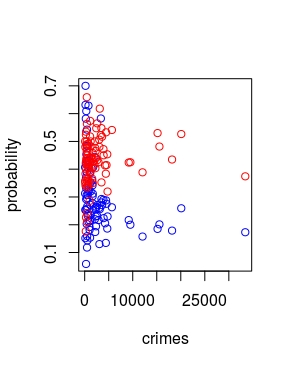
\includegraphics[scale=0.7]{./jpgs/prvc.jpeg}
\caption{Die Arrestierungswahrscheinlichkeiten sind blau gef\"arbt, w\"ahrend die Verurteilungswahrscheinlichkeiten rot gef\"arbt sind.}
\label{fig:nbd}
\end{figure}


\par\smallskip
Die Einflussgr\"o\ss{}en \textit{density} und \textit{area} sind beides r\"aumliche Merkmale. Auch sie wurden in einem Modell zusammengefasst. \\
Wie in Kapitel \ref{sec:preg} bereits erw\"ahnt wurde, liefern Modelle, welche die Variable \textit{density} verwenden, mit die besten Ergebnisse.
In diesem Zusammenhang wurde auch das dichotome Merkmal \textit{region} mit zu dieser Grupperiung gez\"ahlt. \\
Folgende Modelle, die in der unten stehenden Liste \ref{lis:spa} aufgef\"uhrt sind, wurden betrachtet.
Die Ergebnisse dieser Untersuchung liegen in Tabelle \ref{tab:spa} dar. \\
Auch hier ist die selbe Beobachtung wieder zu machen, dass, mit Zunahme der Komplexit\"at der Modelle, sich die Kriterien verbessern.

\begin{itemize}
\item \textsc{mSpatial1: glm.nb($crimes~(density+area)$)}
\item \textsc{mSpatial2: glm.nb($crimes~(density+area)^2$)}
\item \textsc{mSpatial3: glm.nb($crimes~(density+area+region)$)}
\item \textsc{mSpatial4: glm.nb($crimes~(density+area+region)^2$)}
\label{lis:spa}
\end{itemize}

\begin{table}[ht]
\centering
\begin{tabular}{rrrrr}
  \hline
 & df & AIC & SPSE & Devienz\\ 
  \hline
  mSpatial1 & 4.00 & 1462.89 & 3003028556 & 95.0647\\ 
  mSpatial2 & 5.00 & 1463.57 & 3003008479 & 95.00924\\ 
  mSpatial3 & 6.00 & 1460.37 & 3003031244 & 94.74483\\ 
  mSpatial4 & 11.00 & 1444.15 & 3003082475 & 93.6144\\ 
   \hline
\end{tabular}
\caption{\"Ubersicht der Auswertung der Modelle, welche r\"aumliche Einflussgr\"o\ss{}en benutzen.}
\label{tab:spa}
\end{table}

\par\smallskip
Die dritte Gruppierung besteht aus \textit{pctymin} (der Anteil von Minderheiten an der Gesamtbev\"olkerung) und \textit{pctymale} (der Anteil der jungen m\"annlichen Bev\"olkerung (15-24 Jahre)). 
\\
In der vierten Gruppierung wurden alle L\"ohne miteinander kombiniert. \\
Hier wurden jedoch keine weiteren Untersuchungen an der Komplexit\"atszunahme der Modelle gemacht.
Grund daf\"ur ist, dass anhand der ersten beiden Gruppierungsbetrachtungen geschlussfolgert wurde, dass komplexere Modelle auch immer die besseren Akaike-, SPSE- und Devienzwerte haben.
Ausnahme hierbei ist manchmal die Summe \"uber die erwarteten Fehlerquadrate. \\
Stattdessen wurden in diesen beiden Gruppierungen nur die jeweils komplexesten Modelle betrachtet, wie in Liste \ref{lis:pct} und Tabelle \ref{tab:pct} entnommen werden kann.


\begin{itemize}
\item \textsc{mPct: glm.nb($crimes~(pctmin+pctymale)^2$)}
\item \textsc{mTrade: glm.nb($crimes~(1+wsta+wser+wtrd+wfir)^2$)}
\label{lis:pct}
\end{itemize}

\begin{table}[ht]
\centering
\begin{tabular}{rrr}
  \hline
 & df & AIC \\ 
  \hline
mPct & 5.00 & 1612.85 \\ 
  mTrade & 12.00 & 1541.39 \\ 
   \hline
\end{tabular}
\caption{AIC-Werte der komplexen Modelle \textsc{mPct} und \textsc{mTrade}.}
\label{tab:pct}
\end{table}

\par\smallskip
Aus dieser ersten Betrachtung heraus wurde schnell klar, dass besonders die r\"aumlichen Eigenschaften gute Voraussetzungen f\"ur ein geeignetes Modell sind.
In Abbildung \ref{fig:dcc} ist ersichtlich, dass beide Gr\"o\ss{}en proportional zu einander sind und daher gut eine lineare Funktion approximiert werden kann. \\
Auch im Vergleich der Residuenplots ist ersichtlich, dass \textit{density} ein gutes Merkmal ist.
Je mehr Menschen auf engerem Raum wohnen, desto h\"oher ist die Wahrscheinlichkeit eines Verbrechens.
Dies ist insofern schon schl\"ussig, da, wenn es mehr Menschen gibt, automatisch auch gleich die Wahrscheinlichkeit h\"oher sein muss, dass es mehr Delikte gibt, als wenn es weniger Menschen g\"abe.

\begin{figure}
\centering
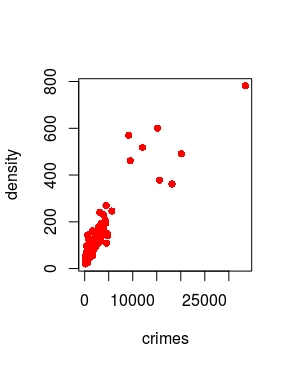
\includegraphics[scale=0.7]{./jpgs/dcc.jpeg}
\caption{Hier ist das Verh\"altnis Verbrechensanzahl / Bev\"olkerungsdichte veranschaulicht.}
\label{fig:dcc}
\end{figure}

Anhand dessen wurde ausgehend von \textsc{mSpatial4} nach weiteren Modellen gesucht, um bessere Werte zu erhalten.
Sie werden in der unten stehenden Tabelle aufgelistet.

\label{lis:pm}
\begin{enumerate}
\item \textsc{m3: glm.nb($rimes ~ 1 + area + density + area:density$)}
\item \textsc{m3Wser: glm.nb($crimes ~ 1 + area + density + area:density + wser$)}
\item \textsc{m3Opt: glm.nb($crimes ~ area + density + wser + area:density + density:wser$)}
\item \textsc{m3Opt2: glm.nb($crimes ~ area + density + wser + area:density + density:wser + prbarr + prbpris$)}
\item \textsc{m3O2: glm.nb($crimes ~ area + density + wser + prbarr + area:density + density:wser + density:prbarr + wser:prbarr + area:wser$)}
\item \textsc{mT: glm.nb($crimes ~ area + density + wser + prbarr + taxpc + area:density + density:wser + density:prbarr + wser:prbarr + area:prbarr + prbarr:taxpc$)}
\item \textsc{mR: glm.nb($crimes ~ area + density + wser + prbarr + region + area:density + density:wser + density:prbarr + wser:prbarr + area:prbarr + density:region + area:wser$)}
\end{enumerate}

\begin{figure}
\centering
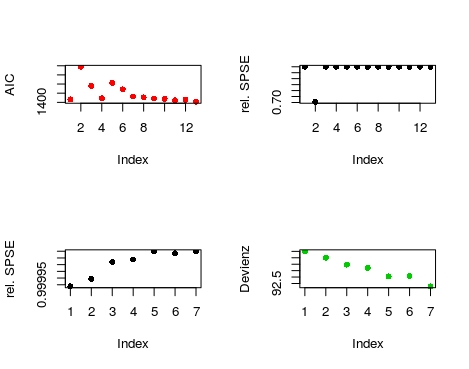
\includegraphics[scale=1]{./jpgs/assdc.jpeg}
\caption{Die Diagramme in der oberen H\"alfte zeigen jeweils die AIC-Werte (links oben) und die zueinander relativierten \hat{SPSE} (rechts oben) auf. Da es bei den \hat{assdc} einen gro\ss{}en Ausrei\ss{}er gibt, sind kaum Unterschiede ersichtlich. Daher wurden die zuletzt hinzugef\"ugten Modelle in der unteren Zeile noch einmal dargestellt. F\"ur die Indexierung der unteren Diagramme siehe \ref{lis:pm}. Die Indexierung der oberen Diagramme wird in Tabelle \ref noch einmal aufgef\"uhrt.}
\label{fig:assdc}
\end{figure}

\begin{table}[ht]
\centering
\begin{tabular}{rrrrr}
  \hline
 & Index & df & AIC & Devienz\\ 
  \hline
  1 & mAll & 17.00 & 1432.29 & 92.88015 \\ 
  2 & m1 & 3.00 & 1789.10 &  2118963611\\ 
  3 & m2 & 5.00 & 1580.94 &  103.9891\\ 
  4 & mSpatial4 & 11.00 & 1444.15 &  93.6144\\ 
  5 & mPct & 5.00 & 1612.85 &  107.5929\\ 
  6 & mTrade & 12.00 & 1541.39 &  99.01972\\ 
  7 & m3 & 5.00 & 1463.57 &  95.00924\\ 
  8 & m3Wser & 6.00 & 1454.43 &  94.50472\\ 
  9 & m3Opt & 7.00 & 1442.88 & 93.96729 \\ 
  10 & m3Opt2 & 9.00 & 1439.20 & 93.71965 \\ 
  11 & m3O2 & 11.00 & 1422.23 & 93.04977 \\ 
  12 & mT & 13.00 & 1428.82 & 93.08855 \\ 
  13 & mR & 16.00 & 1405.77 & 92.27836 \\ 
   \hline
\end{tabular}
\label{tab:assdc}
\end{table}

Bei \textsc{m3Wser} handelt es sich um die Formel, welche die selben Variablen nutzt wie \textsc{m3} und zus\"atzlich \textit{wser}.
In der Betrachtung der Einflussgr\"o\ss{}en aus \textsc{mTrade} war aufgefallen, dass \textit{wser} die beste Verbesserung mit sich bringt. \\
\textsc{m3Wser} wurde daraufhin mit Hife der Funktion \texttt{step()} optimiert.
Das daraus resultierende Modell erhielt den Namen \textsc{m3Opt}. \\
Dieses Modell wurde wiederum dadurch verbessert, indem die beiden Wahrscheinlichkeitsvariablen \textit{prbarr} und \textit{prbpris} hinzugef\"ugt wurden.
Dieses Modell erhielt den Namen \textsc{m3Opt2}. \\
Auch dieses Modell wurde unter der Verwendung von step() erweitert. Das Resultat war Modell \textsc{m3O2}.
Im n\"achsten Schritt wurde eine weitere Variable, n\"amlich \textit{taxpc} (das Pro-Kopf-Steueraufkommen), hinzugef\"ugt.
Durch diese Erweiterung wurde das Modell \textsc{mT} geschaffen. \\
Ein alternatives Modell zu \textsc{mT} soll \textsc{mR} sein: Hier wurde stattdessen \textit{region} hinzugef\"ugt. \\
\par\smallskip
Aus den Diagrammen aus Abbildung \ref{fig:assdc} kann geschlossen werden, dass durch das Hinzuf\"ugen von weiteren Variablen und anschlie\ss{}ende Optimierung die Vergleichswerte AIC und Devienz immer mehr minimieren.
Tats\"achlich verhalten sich die $\hat{SPSE}$-Werte anders.
Dies liegt wahrscheinlich daran, dass AIC und Devienz auch von der Anzahl der Einflussgr\"o\ss{}en beeinflusst werden, was bei den SPSE-Zahlen nicht der Fall ist.
\par\smallskip
Dennoch wurde sich dazu entschlossen, dass das Modell \textsc{mR} das auf diese Herangehensweise ausgesuchte Modell, das beste Modell ist.



% TODO: Diagramm der Kriterienwerte von Modellen hinzufügen, damit ersichtlich wird, dass komplexere Modelle meist die geringereren fehler haben

% TODO: zusammenfassender Residuenplot Übersicht notwendig.

\subsubsection{Vergleich aller Modelle mit jeweils nur einem Merkmal}
Der Ansatz bei dieser Herangehensweise ist, dass jedes Merkmal in ein einzelnes Modell gesetzt wird.
Die daraus resultierenden Modelle werden dann, wie in der ersten Herangehensweise mittels AIC, $\hat{SPSE}$ und Devienz verglichen.
Tabelle \ref{tab:asv} listet die unterschiedlichen Modelle auf und liefert besagte Kriterien, die in Abbildung \ref{fig:asv} in drei Diagrammen dargestellt werden.

\begin{table}[ht]
\centering
\begin{tabular}{rrrrrr}
  \hline
  & name & df & AIC & rel. $\hat{SPSE}$ & Devienz \\ 
  \hline
  1 & mPrbarr & 3.00 & 1584.70 & 0.999975 &  104.8274\\ 
  2 & mPrbpris & 3.00 & 1612.10 & 0.999997 & 107.9817 \\ 
  3 & mPolpc & 3.00 & 1612.10 & 0.999997 &  107.9817\\ 
  4 & mDensity & 3.00 & 1494.42 & 0.9998183 &  96.96636\\ 
  5 & mArea & 3.00 & 1611.75 & 0.9999964 &  107.9404\\ 
  6 & mTaxpc & 3.00 & 1604.40 & 0.9999852 & 107.0648 \\ 
  7 & mRegion & 4.00 & 1594.27 &  0.999976 & 105.6683\\ 
  8 & mPctmin & 3.00 & 1614.37 &  1 & 108.2571\\ 
  9 & mPctymale & 3.00 & 1609.49 & 0.99999 &  107.6686\\ 
  10 & mWcon & 3.00 & 1584.39 &  0.9999629 & 104.799\\ 
  11 & mWsta & 3.00 & 1598.82 &  0.9999806 & 106.4173\\ 
  12 & mWser & 3.00 & 1568.89 &  0.9999449 & 103.1563\\ 
  13 & mWtrd & 3.00 & 1570.84 &  0.9999284 & 103.3589\\ 
  14 & mWfir & 3.00 & 1550.43 &  0.9999175 & 101.349\\ 
   \hline
\end{tabular}
\caption{Auflistung aller Modelle, die nur eine Eingabevariable nutzen.}
\label{tab:asv}
\end{table}
 
\begin{figure}
\centering
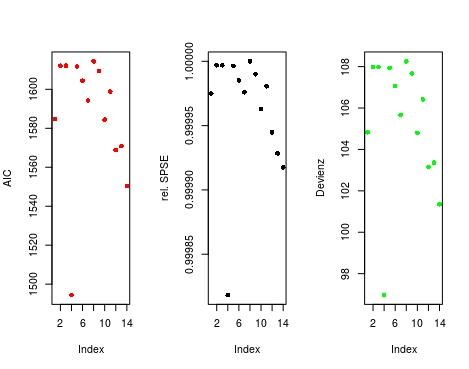
\includegraphics[scale=.7]{./jpgs/asvc.jpeg}
\caption{Veranschaulichung von Akaike-Informationsma\ss{}, $\hat{SPSE}$ und Devienz der Modelle, die jeweils nur eine Eingabevariable besitzen.}
\label{fig:asv}
\end{figure} 
 
Bei Betrachtung von Abbildung \ref{fig:asv} f\"allt auf, dass sich alle drei Kriterien \"ahnlich verhalten.
So besitzt \textsc{mDensity} (Nummer 4) in allen drei F\"allen den gerinsten Wert. \\
Dar\"uber hinaus haben die letzten Modelle, welche die L\"ohne als einzige Eingabe haben, in allen drei Ansichten die n\"achst geringeren Werte.
Hier wurde sich dazu entschieden, die Variablen \textit{density}, \textit{wser}, \textit{wsta}, \textit{wtrd} und \textit{wfir} in ein Modell \textsc{mSingles} als vorl\"aufiges Resultat zusammenzufassen. \\
Dieses Modell wurde nachtr\"aglich noch einmal mit \texttt{step()} optimiert, sodass ein weiteres Modell \textsc{mSinglesOpt} vorliegt.
In Tabelle \ref{tab:svw} wird ersichtlich, dass das beste Modell nach dieser Herangehensweise das Modell \textsc{mSinglesOpt} ist. \\
Tats\"achlich handelt es sich um ein relativ gutes Ergebnis, allerdings sind die Modelle aus der ersten Herangehensweise effektiver.

\begin{table}[ht]
\centering
\begin{tabular}{rrr}
  \hline
 & df & AIC \\ 
  \hline
mSinglesOpt & 8.00 & 1468.70 \\ 
  m3O2 & 11.00 & 1422.23 \\ 
  mR & 16.00 & 1405.77 \\ 
   \hline
\end{tabular}
\caption{AIC-Wert des Ergebnismodells durch Untersuchung der einzelnen Modelle im Vergleich zu den besten Werten aus der erste Herangehensweise.}
\label{tab:svw}
\end{table}

\subsubsection{Verwendung von step() und anschließende Minimierung des Modells}
\subsubsection{strukturierte Suche nach einem geeigneten Modell}
\subsubsection{Verwendung von cor()}
\subsubsection{Die Gewinnermodelle}

\newpage 
\subsection{Simulationsaufgabe}
\paragraph{Beschreibung simulation()}
\paragraph{Auswertung der Ergebnisse}
\subparagraph{einfaches Modell: \textit{mDensity}}
\subparagraph{Ergebnisse mit Gewinnermodell aus der ersten Aufgabe}
Hier leite ich zur Diskussion \"uber.
\newpage

\label{sec:dis}
\section{Diskussion}
\subsection{Auswertung Modellwahl}
Tats\"achlich schneidet im Vergleich zu den anderen drei Herangehensweisen die explorative am besten ab, wie anhand von Tabelle \ref{tab:wic} und Abbildung \ref{fig:wic} nachvollzogen werden kann.
Dies liegt aber auch vor allem daran, dass \textsc{mExplorativ} die geringste Anzahl an Eingabevariablen besitzt.

\begin{table}[ht]
\centering
\begin{tabular}{rrrrrr}
  \hline
  & name & df & AIC & $\hat{SPSE}$ & Devienz  \\ 
  \hline
	1 & mExplorativ & 16.00 & 1405.77 & 0.9999914 & 92.27836 \\ 
	2 & mEinzeln & 8.00 & 1468.70 &  0.999921 & 94.33151\\   
  	3 & mStep & 9.00 & 1457.60 &  1 & 94.97083\\ 
    4 & mCor & 7.00 & 1472.06 &  0.9999654 & 95.23178\\ 
   \hline
\end{tabular}
\caption{Kriterien der vier Gewinnermodelle}
\label{tab:wic}
\end{table}

\begin{figure}
\centering
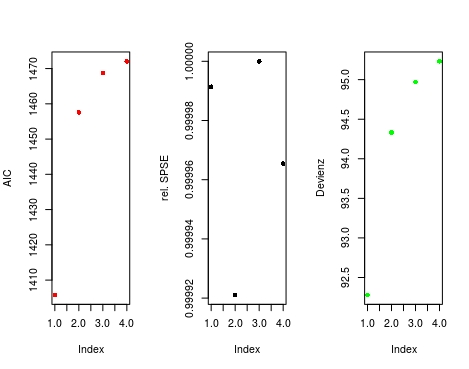
\includegraphics[scale=1]{./jpgs/wic.jpeg}
\caption{Graphische Veranschaulichung der verschiedenen Korrelationswerte.}
\label{fig:wic}
\end{figure} 
Zur Modellwahl muss gesagt werden, dass ein recht gutes Ergebnis mit \textdc{mExplorativ} gefunden wurde.
Auch die anderen gefundenen 'Siegermodelle' sind entsprechend gut.
Anhand der vorgestellten Herangehensweisen k\"onnen also Modelle gefunden werden, welche gute Sch\"atzungen liefern. \\
Zu Beginn der Untersuchung wurde auch die Zielvariable ver\"andert: \\
Statt \textit{crimes} wurden die Werte \text{crimes-per-area} ($cpa$) benutzt.
\begin{equation}
cpa = \frac{crimes}{area}
\end{equation}
Dadurch wurden sehr geringe Werte f\"ur die Kriterien ermittelt.
Dies liegt wohl aber auch an den wesentlich kleineren Bereich, in dem sich dann die Zielgr\"s\ss{}e befindet.

\subsection{Auswertung Simulation}
Bei der Simulationsaufgabe gab es gro\ss{}e Unterschiede betreffend der Ergebnisse.
Vieles war so eingetreten, wie es vermutet wurde.
Allerdings war es auch oft, der Fall, dass die Ergebnisse \"uberhaupt nicht zu den Erwartungen passten.
\\
Besonders in der ersten Aufgabe gab es noch weitere Herangehensweisen, wie z.B. \textit{Mallowc $C_p$}.
Allerdings hatten wir bereits viele andere, bereits bepsrochene Herangehensweisen benutzt.
\newpage


%%%
%%% end main document
%%%
%%%%%%%%%%%%%%%%%%%%%%%%%%%%%%%%%%%%%%%%%%%%%%%%%%%%%%%%%%%%%%%%%%%%%%%%%%%%%%%%

\appendix  %% include it, if something (bibliography, index, ...) follows below

%%%%%%%%%%%%%%%%%%%%%%%%%%%%%%%%%%%%%%%%%%%%%%%%%%%%%%%%%%%%%%%%%%%%%%%%%%%%%%%%
%%%
%%% bibliography
%%%
%%% available styles: abbrv, acm, alpha, apalike, ieeetr, plain, siam, unsrt
%%%
\bibliographystyle{plain}
\bibliography{chapters/sources}
\section{Literaturverzeichnis}
\begin{itemize}
\item Badi H. Baltagli, estimating an economic model of crime using panel data from North Carolina, journal of applied econometrics
\item Cornwell C, Trumbull WN. 1994. Estimating the economic model of crime with panel data. Review of
Economics and Statistics 76: 360 - 366
\item Ehrlich I. 1973. Participation in illegitimate activities: a theoretical and empirical investigation. Journal of Political Economy 81: 521–567.
\end{itemize}


\end{document}
%%% }}}
%%% END OF FILE
%%%%%%%%%%%%%%%%%%%%%%%%%%%%%%%%%%%%%%%%%%%%%%%%%%%%%%%%%%%%%%%%%%%%%%%%%%%%%%%%
%%% Notice!
%%% This file uses the outline-mode of emacs and the foldmethod of Vim.
%%% Press 'zi' to unfold the file in Vim.
%%% See ':help folding' for more information.
%%%%%%%%%%%%%%%%%%%%%%%%%%%%%%%%%%%%%%%%%%%%%%%%%%%%%%%%%%%%%%%%%%%%%%%%%%%%%%%%
%% Local Variables:
%% mode: outline-minor
%% OPToutline-regexp: "%% .*"
%% OPTeval: (hide-body)
%% emerge-set-combine-versions-template: "%a\n%b\n"
%% End:
%% vim:foldmethod=marker
